\chapter[\paperItitle]{\texorpdfstring{%
                \paperItitle}{%
                \paperItitle}}

\label{ch:ot}
\paperRemark{\paperIref}

{

\section{Introduction}
\label{sec:introduction}

The amount of connected devices deployed are increasing. Connected devices can take the form of sensors and actuators in home, industrial or smart-city settings. They can also be connected medical devices or connected cars. In particular, we see a trend towards usage of very large IoT infrastructures consisting of a huge number of heterogeneous devices  \cite{Vogler2016} . Managing such heterogeneous infrastructures is challenging and an issue that has been addressed in several recent research works \cite{Lanza2016} \cite{DIAZ201699}. 

Large IoT infrastructures must also be managed and controlled from a security perspective. An expectation of such a system is secure communication as well as authentication and authorization, thus credentials for the IoT devices must be issued and updated \cite{Roman2011}. Credential management can be done using standard protocols and procedures such as IKE and HIP \cite{rfc5996}\cite{Said2012} and these procedures are working well as long as a single organization is controlling the infrastructure.

However, transferring ownership of a complete infrastructure is more complicated. One core problem is backward and forward secrecy with respect to the old and new owners. The new owner of the system shall not be able to deduce anything the old owner has done before the transfer of ownership. Vice versa, the old owner shall not be able to learn anything of what the new owner does after the transfer of ownership. Furthermore, there should not be any time slot when a single IoT unit is under control of both the old and new owners simultaneously. 

The problem of IoT infrastructure ownership transfer is related to the problem of transferring ownership of RFID tags, a topic that has been extensively treated in the literature in the past \cite{taqieddin2018tag}. Especially, it is related to the problem of group ownership transfer of RFID tags \cite{zuo2010changing}\cite{kapoor2011multi}\cite{He2014}. Inspired by these earlier works we have looked into the ownership transfer problem again, now from the IoT infrastructure perspective.  Similar to some previous work for tag ownership transfer, we are interested in finding symmetric key solutions not being dependent on public key support on the IoT side. This allows ownership transfer also for very resource constrained IoT units in the system\cite{Eisenbarth2007}. By analyzing the security expectations for such scenario, we have identified the main security requirements for IoT infrastructure ownership transfer. The requirements then allowed us to suggest a suitable ownership transfer model based on the assumption of trusted third party, or what we refer to as a ‘’Reset Server’’ (RS) present in the system. We present a protocol for ownership transfer under this model. 
Our ownership transfer protocol meets the identified requirements, and has not previously presented in the literature. Our suggested approach does not need active involvement of the RS during normal operation, a property we see as a major advantage. Furthermore, the RS does not need to store individual IoT device keys, reducing the storage requirements of the RS.

The main contributions of the paper are the following
\begin{itemize}
    \item We analyse the IoT infrastructure ownership transfer problem and conclude that it has similar but not equal security requirements compared with those identified in previous analyses of group ownership transfer for tags.
    \item We suggest a novel IoT infrastructure ownership transfer model and protocol for symmetric keys based on the usage of an RS in the system.
    \item We present a proof of concept implementation and performance evaluation of the proposed ownership transfer scheme.
    \item We make a security analysis of the proposed ownership transfer protocol using both Tamarin Prover and logical reasoning.
\end{itemize}

We proceed as follows: we discuss related work (\S \ref{sec:ot:RelatedWork}), we introduce our system model (\S \ref{sec:ot:System}), identify security requirements and give a problem definition (\S \ref{sec:ot:threat-model}), we present our ownership transfer model and protocol design (\S \ref{sec:ot:Solution}), we describe our proof-of-concept implementation including performance benchmarks (\S \ref{sec:ot:Implementation}), we perform  security analysis of the proposed transfer protocol (\S \ref{sec:ot:analysis}) and conclude (\S \ref{sec:ot:Conclusion}).

\section{Related work}
\label{sec:ot:RelatedWork}

Protocols for ownership transfer have been studied in several fields. Both recently for IoT devices and earlier for RFID-tags. IoT infrastructures and RFID systems are not equal but share some characteristics. RFID-tags and IoT systems are deployed in large numbers and efficient management of a large number of devices is necessary. IoT devices might have constrained resources and RFID-tags typically even less resources for computation and storage. IoT units though have connectivity, usually wireless, and the ability to initiate communication with external entities. RFID-tags however are only capable of responding to requests.
RFID-tags can only be read and written to locally, a reader must be in physical proximity to the RFID-tag to be able to communicate with the device. An IoT device can however receive communication originating practically anywhere, this creates a bigger attack surface on IoT devices since an attack on the system can, in theory, originate from anywhere on the planet.

\subsection{IoT Ownership Transfer}
Internet of Things (IoT) are a very wide category of devices with the common property that they are connected to a network in some way. When ownership transfer is studied in the realm of IoT devices authors often have different views of what types of devices constitute an IoT device. Devices considered can be connected medical equipment, wearables, smart consumer electronics such as fridges and CCTV-cameras. Other devices that are often grouped into IoT are sensor networks, building automation and connected equipment for industry. 

Tam and Newmarch state the problem of transferring ownership in  \cite{tam2004protocol} for Ubiquitous Computing Networks, a term that predates IoT. They define the term ownership and provide requirements for an ownership system. They also provide an example of an ownership transfer protocol. The protocol is based on public-key cryptography and defines how two parties transfer the ownership of a device. 

Khan et. al. discuss ownership transfer for connected consumer products \cite{Khan2019}. The focus of the ownership transfer process is less about re-keying the device and more about preserving privacy for information stored on the device. They also propose a novel idea of  how to automatically start the ownership transfer process by detecting changes in the environment to determine if the device has been sold or given away. 

Pradeep and Singh propose a protocol in \cite{Pradeep2013} utilizing a trusted third party that they call a Central Key Server. The protocol requires physical proximity when the ownership transfer process is about to take place. The protocol does not specify exactly what type of IoT device that is considered, but only one device is transferred during each execution of the protocol.

\subsection{Ownership Transfer Protocols for RFID-tags}
The subject of secure ownership transfer has been studied in the field of RFID technology since 2005 \cite{saito2005reassignment}. In the paper "Tag Ownership in RFID systems: Survey of Existing Protocols and Open Challenges"\cite{taqieddin2018tag} the authors list the research done in the field from 2005 to 2018. The authors also group protocols by features; Group transfer protocols and individual tag transfer protocols, trusted Third Party (TTP) protocols, and protocols where only the new and current owner take part. Lastly EPC-C1G2 \cite{epc-c1g2} compliant protocols and protocols that require more resources from the tags. The first papers for RFID-tag ownership transfer generally suffered from not satisfying some important security requirements. The early Satio paper \cite{saito2005reassignment}, does for instance not provide forward and backwards secrecy for the owners. 
%Old- and new-owner secrecy in the context of ownership transfer protocols means that the old owner shall learn nothing about what the new owner does with the system after a transfer of ownership. The new owner shall in turn learn nothing about what the old owner has done. This includes being able to decrypt messages, see commands executed and data that has been generated i.e. the property that the new owner does not learn anything about past owner IoT unit information or communication and similar for the old owner with respect to the new one.

We are considering a model with IoT ownership transfer with the assistance of a trusted third party node, the so-called ''Reset Server'' (RS) (see Section \ref{sec:ot:System} and Section \ref{sec:ot:Solution}). This entity has a very similar role as a TTP in RFID ownership transfer solutions. However, {\em different} from prior art work, we think that for IoT infrastructures, one would like to avoid the TTP to actual {\em choose} the credentials for the devices in the system but merely ''supervise" the transferring process. This has the main advantage that the RS, unlike the TTP in prior-art solutions, will not have complete knowledge of the final device credential after completing the ownership transfer process. TTP based protocols in prior-art are the ones that most closely resemble the model we consider and we will in the related work summary below, focus on TTP based protocols.” 

\subsection{RFID Single ownership transfer}
Much work has been done for owner transfer of single RFID-tags. Since we consider group transfer of IoT devices these protocols are mainly mentioned for completeness sake. Protocols that are intended for EPC-compliance are often forced to use non-standard solutions due to the extremely constrained nature of EPC-compliant RFID-tags. One such scheme can be found in \cite{CAO201647}. 
The protocols that are not restricted by EPC-compliance often make use of standard cryptological functions such as symmetric ciphers and hash functions. One example of an ownership transfer protocol using a TTP can be found in \cite{zhou2012simultaneous}.



\subsection{RFID Group ownership transfer}
Several group transfer protocols with a TTP have been proposed in the literature \cite{kapoor2011multi} \cite{zuo2010changing}  \cite{SUNDARESAN2015112} \cite{He2014} \cite{BagheriAS18}. The design goals of the different protocols are not uniform. They do not work with the very same security requirements. They also differ with respect to that one solution wants to achieve EPC-C1G2 compliance \cite{SUNDARESAN2015112} and another want to have a group of nodes to switch ownership simultaneously for instance \cite{zuo2010changing}.

A core characteristic we expect from an ownership transfer protocol, is backward and forward secrecy. This is not offered by the protocol suggested by Sundaresan et al. \cite{SUNDARESAN2015112}. The group transfer protocol by Kapoor \cite{kapoor2011multi} is an extension of an earlier variant for singe tag transfer \cite{Kapoor2008}. Even if this is a simple and rather straightforward protocol, these protocols were later shown by Bagheri et al \cite{BagheriAS18} to be vulnerable to de-synchronization attacks (due to the simple fact that the message exchange between the TTP and the tag was not authenticated). The authors in \cite{BagheriAS18} also showed how to fix these shortcomings, but unlike our suggested protocol, their solution is dependent on a direct session between the tag (the IoT unit in our case) and the TTP. They also give the full power to the TTP that must have access to all key information (both the old and the new).

Inspired by an earlier work on grouping proofs for RFID tags \cite{Burmeister2008}, Zuo proposed a new TTP based protocol for RFID ownership transfer \cite{zuo2010changing}. Similar to the earlier grouping proof protocols, the design goal is to provide a proof of the ownership transfer of all tags in a group {\em simultaneously}, i.e., without the need of having connection to the back-end system representing the tag owner during the ownership switch. This means that the ownership transfer interactions only take place locally between the tag reader and the tags in the group connected to this reader. Later, the back-end system just can verify that the transfer has occurred. In and RFID system scenario this has some communication overhead reduction advantages but not in a system scenario with distributed IoT units.  Hence, the off line requirement makes the ownership transfer unnecessarily complex for the IoT scenario we are considering. Furthermore, similar to other ownership protocols, the TTP is given full power by selecting all the new credentials using the solution in \cite{zuo2010changing}. 

In \cite{He2014} another group ownership transfer protocol was proposed. This protocol shares our design goals with respect to forward and backward secrecy. Furthermore, it allows arbitrary location and grouping of tags based on group keys. This is a property most suitable also for IoT infrastructures. However, similar to other prior art, the solution in \cite{He2014} gives the TTP full knowledge of the key information. It also must has active sessions with all tags taking part in the ownership transfer process. Our protocol does not have these two limitations.

\section{System model and assumptions}
\label{sec:ot:System}

This paper considers IoT deployments as seen in Figure \ref{fig:system_0}, comprised by a large number of IoT nodes deployed  managed by a Device Management Server (DMS) owned and operated by some entity. The considered system can be part of an Internet connected industrial automation system or smart sensors deployed to monitor the environment for e.g. pollution. The IoT nodes communicate with the DMS through intermediate parties and the last hop to the IoT nodes can be assumed to be wireless communication. The IoT nodes can be resource constrained nodes, this means that their hardware capabilities; such as processing power and memory are limited. The IoT devices are capable of symmetric cryptography, asymmetric cryptography is not feasible for these devices, mainly due to the increased bandwidth required. The used wireless communication technology is limited in bandwidth and latency. The DMS is assumed to be a server, in a cloud environment or located on premise in the organization. 

\begin{figure}
\centering
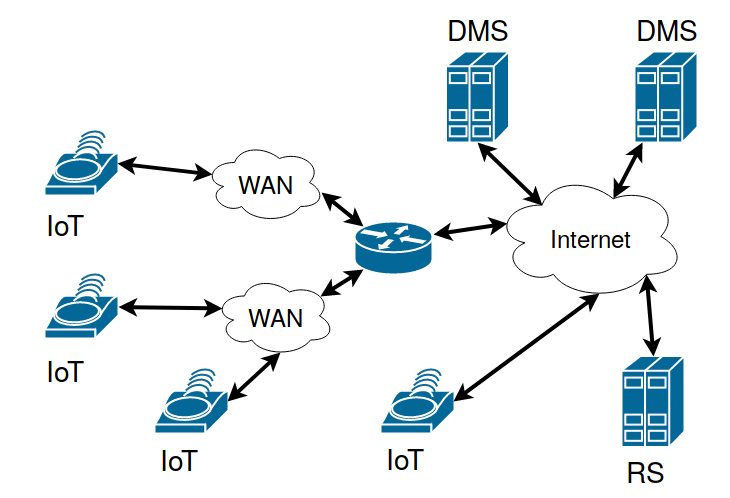
\includegraphics[width=200pt]{papers/ot/images/ot-fig-1.png}
\caption{An overview of the considered system}
\label{fig:system_0}
\end{figure}

In the scenario depicted in Figure \ref{fig:system_0}, the different IoT units are connected to the Internet and consequently vulnerable to all kinds of network based attacks. Hence, it is important that the IoT units are properly authenticated and that only well protected communications are allowed over the Internet and over the wireless network. In particular, independent of Internet access technology, there must be credentials in place on the IoT units so that they can securely perform mutual authentication with the back-end system. 
For an ownership transfer to take place we assume that there exists another organization, with its own DMS, to transfer the ownership to. 


We furthermore assume the existence of a trusted third party in the form of an RS. RS i operated by an organization that both organizations trust to a high degree. The RS will facilitate the ownership transfer process.
The RS and DMS are not constrained in what types of cryptographic operations they can do i.e. asymmetric cryptography is possible. We also assume that the DMS servers and RS can exchange keys and authenticate each other, possibly with a PKI. The cryptographic functions are assumed to be secure.

\section{Adversarial model and problem description}
\label{sec:ot:threat-model}
\subsection{Adversarial model}
\label{sec:ot:adversary}
Similar to many existing work in IoT and cloud security, we assume that the adversary is acting according to the Dolev-Yao adversarial model \cite{Dolev1981}. This means that an attacker is able to intercept, delete, change order or modify all messages sent over the communication channel between any entity. The adversary can also destroy messages, but is not able to break cryptographic functions. Furthermore, we assume the IoT nodes are placed into an environment such that physical attacks from an insider adversary (such as the current owner) have to be considered while the DMS and the RS are assumed to be in a secure location or in protected isolated environments protected from both external and insider software attacks.

With respect to the direct physical attacks on the IoT units, we assume that an adversary as well as the old and new DMS are able to compromise, with a given effort, some or a limited number of IoT units through direct physical attacks on the devices. Here a compromised node refer to a node where the attacker has full control of the execution environment as well as volatile and persistent storage units of the device. Such a model is motivated by the fact that the needed effort for direct physical attacks is at least proportional to the number of compromised units.  Attacks from the current or new owner on a large scale can be very hard to perform in practice due to hardware protection mechanisms on the IoT units for instance.
\subsection{Trust model}
 The RS is assumed to be ‘’honest but curious’’ \cite{Oded2009}, which means the RS will be a legitimate  participant in protocol interactions. It will not deviate from the defined protocol, but will attempt to learn all possible information from legitimately received messages. The Old Owner and the New Owner are assumed to not fully trust each other, i.e. the Old Owner has interest in learning the secrets used by the New Owner. Similar, the New Owner would like to get hold of the secrets used by the Old Owner.

\subsection{Requirements}
\label{sec:ot:requirements}
Given the previously introduced adversary model, we have looked over the general ownership transfer security requirements identified in previous work on RFID tags \cite{taqieddin2018tag} and adapted them to our system and adversary model: 
\begin{labeling}{R11.}
%\item [R1.] \textbf{Ownership transfer security:} The protocol shall net allow any outside entity to learn credentials for any party in the system.
\item [R1.] \textbf{IoT unit impersonation security:} The protocol shall not allow an adversary to impersonate legitimate IoT units during or after ownership transfer.
\item [R2.] \textbf{Old DMS impersonation security:} The protocol shall not allow an adversary or the new DMS to impersonate the old DMS.
\item [R3.] \textbf{New DMS impersonation security:} The protocol shall not allow an adversary or the old DMS to impersonate the new DMS.
\item [R4.] \textbf{RS impersonation security:} The protocol shall not allow an adversary, any IoT unit or any DMS in the system to impersonate the RS.
\item [R5.] \textbf{Reply attack resistance:} The protocol shall be resistant against attacks where an adversary tries to complete sessions with any entities in the system by replaying old, observed messages.
\item [R6.] \textbf{Resistance to Man-in-the-Middle attacks (MitM):} The protocol shall not allow insertion or modification of any messages sent between trusted entities in the system.
\item [R7.] \textbf{Resistance to de-synchronization attack:} The protocol should not allow the IoT units and the new or old DMS to enter a state where necessary secure communications is prevented by a credential mismatch. 
\item [R8.] \textbf{Backward security:} During and after an IoT ownership transfer, the new owner shall not be given access to any secrets allowing the new owner to get access to any identities or confidential information used in past sessions between the old DMS and the IoT units.
\item [R9.] \textbf{Forward security:} During and after an IoT ownership transfer, the old owner shall not be given access to any secrets allowing the old owner to get access to any identities or confidential information used in sessions between the new DMS and the IoT units.
 \item [R10.] \textbf{No double ownership:} There shall not be any time period during the ownership transfer process when both the old and the new owner has control over an IoT unit in the system.
\end{labeling}

In addition to these requirements, our adversary model does not imply full trust in the RS and we also take into account the risk of that IoT units might be compromised through direct physical attacks. These two assumptions give the following additional two requirements:

\begin{labeling}{R12.}
\item [R11.] \textbf{Protection of new credentials :} After the completion of the ownership transfer, the RS shall not have knowledge of the new IoT credentials and shall not be able to set impersonate the new DMS or have access to secure sessions between the new DMS and the IoT units in the system.
\item [R12.] \textbf{IoT compromise resilience:} A successful compromise of an IoT unit by an external or internal adversary shall only give the adversary the power to impersonate this single IoT unit in the system and not impersonate or break any secure sessions between other, non-compromised IoT units in the system and the new DMS.
\end{labeling}

In many IoT infrastructures, some IoT units are placed in local networks not publicly open but they are accessible by the owner system only. In our case, this means that the current DMS can access the units but not for instance an external entity like the RS. Opening up the system and allowing direct interactions between all IoT units in the system and the RS is a potential security risk. Hence, we have the following additional requirement on the system solution:

\begin{labeling}{R13.}
\item [R13.] \textbf{IoT unit isolation:} An ownership transfer shall not require any direct interactions between the IoT unit and the RS but only between the IoT unit and the DMS (old or new) in the system.
\end{labeling}
\subsection{Problem statement}
\label{sec:ot:problem}
We want to transfer the ownership of a set of deployed IoT devices from one entity to another. Each IoT device has some form of credentials that it shares with a remote entity. Ownership is defined as holding the credentials of the individual IoT-nodes. Ownership transfer then is the process of updating the credentials from keys shared with the old owner to keys shared with the new owner. We want to find an ownership transfer protocol and solution secure under the previously defined threat model and which meets the identified security requirements in Section \ref{sec:ot:requirements}.

\section{IoT infrastructure ownership transfer model and protocol design}
\label{sec:ot:Solution}
The ownership transfer process can, according to our solution, be divided into three phases:
\begin{itemize}
\item Deployment
\item Ownership transfer preparation
\item Ownership transfer
\end{itemize}
In the deployment stage the RS and the first owner provisions keys to the individual devices, the devices are then deployed.

In the ownership-transfer preparation phase, the owner, now called old owner, and the new owner signs a list of all devices that shall be transferred and forwards this list to the RS. The RS then distributes the needed keys for the transfer and generates an ownership transfer token as well as the individual keys to the new owner.

In the final ownership transfer stage, the old owner sends the ownership transfer token to the IoT units. After receiving the token the IoT devices verify and decrypt the token. The information in the token is used to contact the new owner. The new owner and the IoT units then authenticate each other and new credentials are provisioned to the IoT devices. The detailed protocol description is done in the subsection below, using terminology defined in Table \ref{tab:notation}, and illustrated in Figure \ref{fig:proto-2}. The steps from Figure \ref{fig:proto-2} are references by bold numbers e.g. \textbf{(1.1)}.

\begin{table}

\begin{tabularx}{\textwidth}{l m{9cm}}
\hline
      $DMS_{old}$ & Old Device Management Server  \\
      $DMS_{new}$ & New Device Management Server  \\
      $RS$ &Reset server  \\
    
      $Sign(P, d)$ & Digital signature of data $d$ by party $P$.  \\
      $E(k,m)$  & Symmetric encryption of message $m$ with key $k$.  \\
      $D(k,c)$  & Symmetric decryption of ciphertext $c$ with key $k$.  \\
      $MAC(k,m)$  & Message Authentication Code of message $m$ with key $k$.  \\
      $PRF(s)$ & Pseudo-random function with seed $s$, generating  \\
               & a pseudo random key. \\
    
      $IoT_i$  & IoT device number $i$.  \\ 
      $ID_i$  & Identifier of IoT device $i$. \\
      $ID_{new}$ & Identifier of $DMS_{new}$.  \\ 
      $URL_{new}$ & Uniform resource locator to $DMS_{new}$.  \\ 
      $K_i$ & Key for IoT device number $i$, shared with $RS$  \\ 
      $KR_E$ & Reset-key used for encryption.  \\ 
      $KR_M$ & Reset-key used for message authentication.  \\
      $KO_i$ & Owner-key for IoT device number $i$, divided into two parts  $KO_i = \{KO_{i1}, KO_{i2}\}$  \\
      $K_{RS}$ & Master-key for $RS$ used for deriving $K_i$.  \\

      $N$ & Ownership-transfer nonce.  \\
      $Ctr_i$ & Counter for node $i$ is used for verifying freshness  of nonces.  \\
      $Ctr_{RS}$ & Counter for $RS$, incremented at every ownership transfer. Used for verifying freshness of nonces.\\
      $KS_i$ & Ownership transfer key for node $i$ composed by: $KS_i = PRF( K_i || N || Ctr_{RS})$ \\
       $T$ & Ownership-transfer token, calculated by:  \\
          & $T = E(KR_E, ID_{new} || URL_{new} || N || Ctr_{RS} ||$ \\
          &$ MAC(KR_M, ID_{new} || URL_{new} || N || Ctr_{RS} ))$  \\
      $PSK_i$ & DLTS-PSK for IoT device $i$, generated by $PSK_i = PRF(KS_i || KO_{i2})$ \\
      \textbf{ID} & List of IoT device identities \textbf{ID} $= \{ID_1, ID_2, ... , ID_i\}$ \\
      \textbf{ID-K} & List of pairs of  IoT device identities and $KO_{i2}$:  \\
                    &  \textbf{ID-K} $= \{(ID_1,KO_{12}),  ... , (ID_i, KO_{i2})\}$ \\
      \textbf{K} & List of keys $K_i$ \textbf{K} $= \{K_1, K_2, ... , K_i\}$ \\
      \textbf{KO} & List of owner-keys $KO_i$, \textbf{KO} $= \{KO_1, KO_2, ... , KO_i\}$ \\
      \textbf{KS} & List of keys $KS_i$, \textbf{KS} $= \{KS_1, KS_2, ... , KS_i\}$ \\
      \textbf{ID-KS} & List of IoT device identities and keys: \\
                     &  \textbf{ID-KS} $= \{(ID_1, KS_1), ... , (ID_i, KS_i)\}$ \\
          \hline
%\end{tabular}
\end{tabularx}
\caption{Notations used in protocol description.}
\label{tab:notation}
\end{table}

\subsection{Deployment}


$RS$ generates the keys $KR_E$, $KR_M$ and $K_{RS}$. $RS$ provides each IoT device with a unique identifier $ID_i$. $K_{RS}$ is then used to generate $K_i$ for each $IoT_i$ by calculating $K_i = PRF(K_{RS} || ID_i)$. Each device $IoT_i$ is provided with the corresponding $KR_E$, $KR_M$, $ID_i$ and $K_i$. After transferring the keys $RS$ can discard all keys $K_i$. $RS$ sets its counter $Ctr_{RS} = 0$ and all IoT devices counters $Ctr_i$ are also set to zero. These counters are used to verify the freshness of the ownership tokens later on.
The first owner, $DMS_{old}$, takes control of the system and provides the owner-key $KO_i = \{KO_{i1}, KO_{i2}\}$ to each device $IoT_i$. The system is then ready for deployment and regular use, with $KO_i$ used for securing the communication with $DMS_{old}$. 

\subsection{Ownership transfer preparation}
The ownership transfer process starts with a preparation phase with interactions between the $RS$, $DMS_{old}$ and $DMS_{new}$. $DMS_{old}$ creates a list of all IoT device identities $ID_i$ called \textbf{ID} and a list of identities and partial keys $\{ID_i, KO_{i2} \}$ called \textbf{ID-K} that shall switch owner \textbf{(1.1)}. The list of identities is signed $Sign(DMS_{old}, \mathbf{ID})$.
Both lists are sent to $DMS_{new}$ \textbf{(1.2)}, $DMS_{new}$ first verifies the signature of the list, the list of identifiers are then signed by $DMS_{new}$. 

The result is $Sign(DMS_{new}, Sign(DMS_{old}, \mathbf{ID}))$, \textbf{ID-K} is kept by $DMS_{new}$ \textbf{(1.3)}. The list \textbf{ID} is sent to $RS$, to prove that ownership transfer shall take place and that both $DMS_{old}$ and $DMS_{new}$ are agreeing to the transfer \textbf{(1.4)}. $DMS_{new}$ also sends its identifier and URL to $RS$.
After verifying that the list \textbf{ID} is correctly signed by both $DMS_{old}$ and $DMS_{new}$ \textbf{(1.5)}, $RS$ can start the ownership transfer protocol. 

\subsection{Ownership transfer}
$RS$ start the ownership transfer process by re-generating the keys $K_i$. A nonce $N$ is generated, that together with $Ctr_{RS}$ is used to generate the individual ownership transfer keys $KS_i = PRF(K_i || N || Ctr_{RS})$ \textbf{(2.1)}. The list of ownership transfer keys \textbf{ID-KS} is sent to $DMS_{new}$ \textbf{(2.2)}. The $RS$ creates the ownership transfer token $T$, with information needed by the IoT devices, authorizing an ownership transfer and information for how to do it. $T = E(KR_E, ID_{new} || URL_{new} || N || Ctr_{RS} || \\ MAC(KR_M, ID_{new} || URL_{new} || N || Ctr_{RS} ))$
$RS$ sends the token $T$ to $DMS_{old}$ \textbf{(2.3)}.
$DMS_{old}$ forwards the Ownership Transfer Token $T$ to all IoT devices \textbf{(2.4)}. The devices decrypts $T$ with $KR_E$ and verifies the MAC with $KR_M$. If the MAC verification succeed, the freshness of the nonce is checked by verifying $Ctr_{RS} > Ctr_i$ (\textbf{2.5}). After these checks each IoT device $IoT_i$ can compute the ownership transfer key $KS_i = PRF(K_i || N || Ctr_{RS})$ (\textbf{2.6}). With $KS_i$ and $KO_{i2}$ the IoT devices can connect to $DMS_{New}$ using DTLS-PSK\cite{rfc7925}. The parameters used are PSK-ID = $ID_i$ and PSK = $PRF(KS_i || KO_{i2})$ (\textbf{2.7}). After a successful contact has been made with $DMS_{new}$ $IoT_i$ destroys $KO_{i1}$ (\textbf{2.8}). $DMS_{new}$ then generates a new key $KO'_i$ (\textbf{2.9}). The new key $KO'_i$ is sent to $IoT_i$, that also sets $Ctr_i$ to the received value $Ctr_{RS}$(\textbf{2.10}). After $DMS_{new}$ has provisioned new keys to all IoT devices the ownership transfer process is concluded. $DMS_{new}$ can securely communicate with all IoT devices using the new keys $KO'_i$.

\begin{figure*}[ht]
\centering
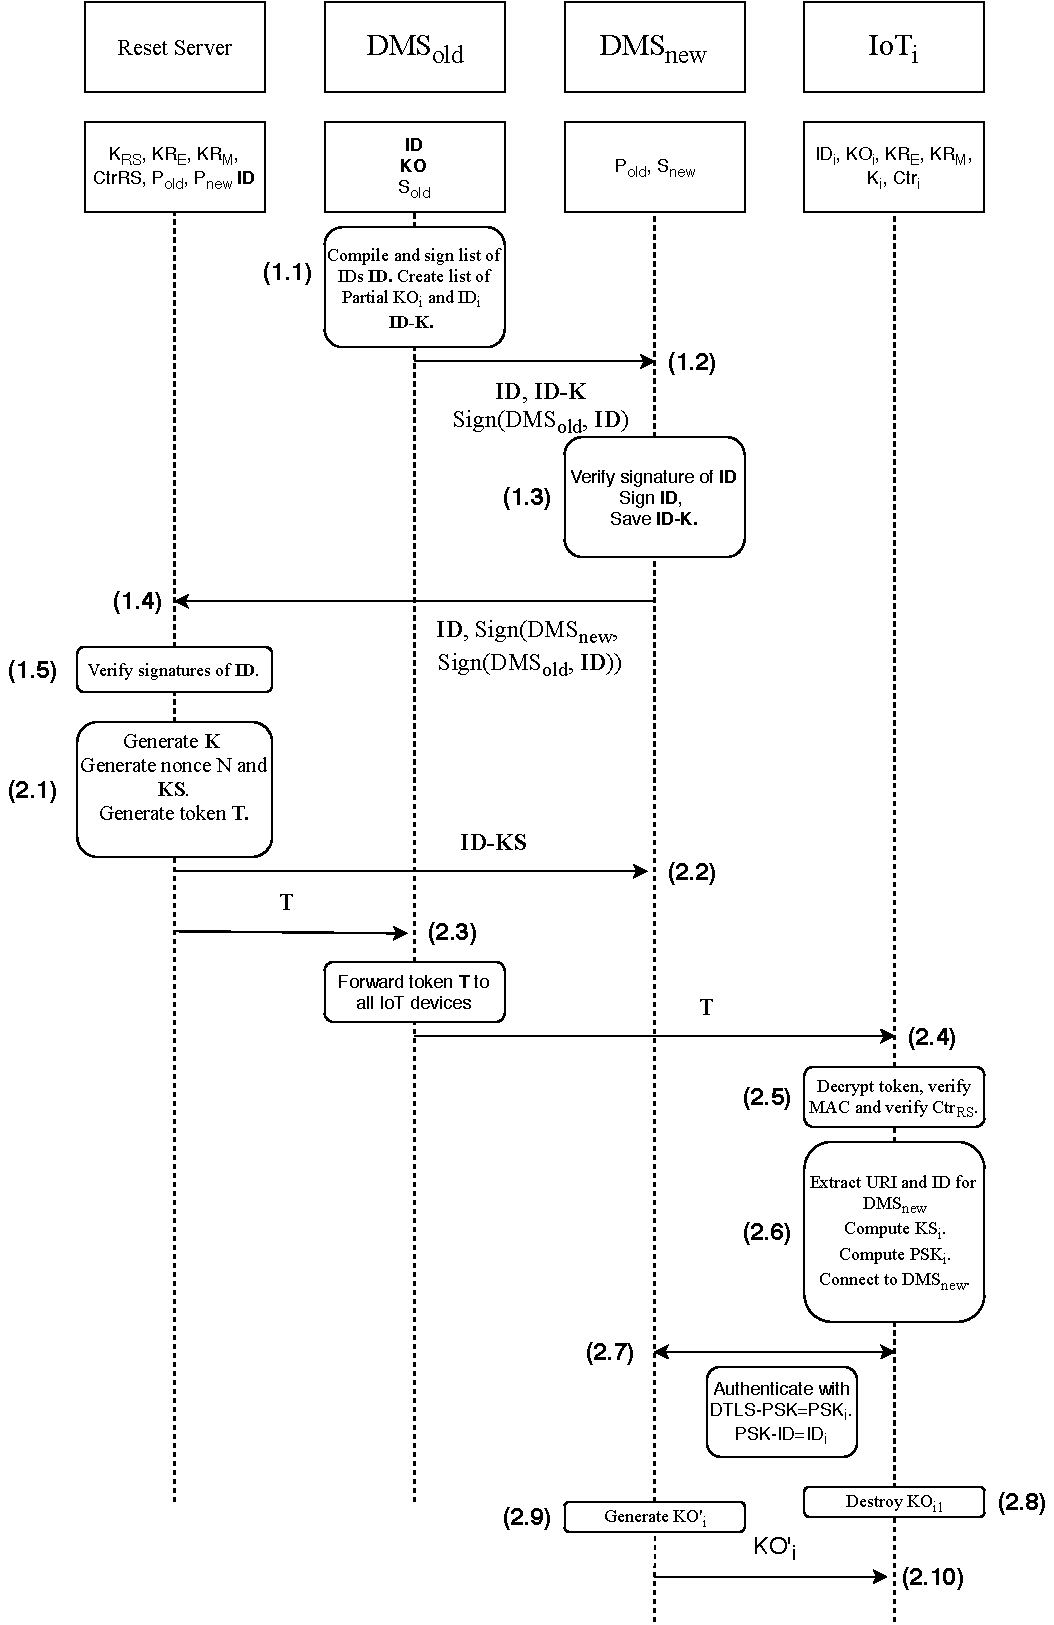
\includegraphics[scale=0.545]{papers/ot/images/ot-proto-2.pdf}
\caption{Messages and computations done during the ownership transfer.}
\label{fig:proto-2}
\end{figure*}

\subsection{Handling of ownership transfer failures}
\label{sec:ot:failures}
 In the previous sections we have described the ownership transfer process in detail. However, there is a risk that the ownership transfer succeeds for one set of IoT units but not for another set due to communication errors or similar. Such situation will be detected by the $DMS_{New}$ as it will notice that it has not been able get in contact and authenticate some units part of the IoT transfer list given in step 1.2. $DMS_{New}$ can first retransmit the ownership transfer token $T$ to the devices that has not changed ownership. Some protocols provide a mechanism of notifying a sender that a message has been received. Such a mechanism can be used to verify the proper delivery of $T$. If $T$ has been delivered but an IoT device still does not connect to $DMS_{New}$ the issue lies with the device $IoT_i$, that situation will have to be resolved by $DMS_{Old}$ before a new attempt can be made.  In such situation, it is possible is for $DMS_{New}$ to issue a ''recovery'' procedure by sending a signed list of missing units back to $DMS_{Old}$, which then will be requested to contact each of the missing IoT units (still under ownership of $DMS_{Old}$) over a mutual authenticated DTLS channel re-sending the transfer token, $T$. Such procedure can be repeated, until the whole set of IoT units are successfully transferred to $DMS_{New}$.

\section{Implementation and experimental evaluations}
\label{sec:ot:Implementation}
We have implemented our proposed protocol for an IoT environment running Contiki-NG\footnote{ \url{https://github.com/contiki-ng/contiki-ng}}. Contiki-NG is a light-weight operating system designed for constrained devices. We have used some other protocols to structure our data. Most significantly we use COSE \cite{rfc8152} to encode and encrypt the ownership transfer tokens. We assume secure communication between the $RS$, $DMS_{old}$ and $DMS_{new}$. The connections to the IoT devices are secured with DTLS\cite{rfc6347}. 

We have designed the system to use the REST-model\cite{fielding2000representational}. Sending the ownership transfer token to the IoT device is done with a PUT operation to /transfer-ownership. The IoT device then sends a GET message to /key to receive the new keys $K'_i$ and $KO'_i$. 


\subsection{Test Setup}
The evaluated scenario is executed on the following setup. One Desktop PC running the $RS$, $DMS_{Old}$ and $DMS_{New}$. The PC is connected to a Border-Router that acts as an IEEE 802.15.4 network interface. We have used four Zolertia Firefly-A development boards\footnote{\url{https://github.com/Zolertia/Resources/wiki/Firefly}} that are going to transfer from owner $Old$ to $New$. The IoT devices are based on the cc2538 system on chip made by Texas Instruments\cite{instruments2015cc2538}. They have an ARM Cortex-M3 CPU clocked at 32MHz together with 32KB of RAM and 512KB of flash. Connectivity is provided by an IEEE 802.15.4 radio providing about 100Kb/s of bandwidth. 

\subsection{Test Scenario}
The test scenario consists of an initial setup phase where keys are distributed to the individual IoT nodes and an ownership transfer phase. The initial setup phase is not in scope for the performance evaluation, only the ownership transfer process is included. We ran the ownership transfer scenario, of the four IoT devices, ten times.

\subsection{Ownership transfer time}
In order to evaluate the efficiency of our proposed scheme from a system perspective we timed the entire ownership transfer process. We measured the time elapsed from that the $RS$ sends out the token $T$ to when all IoT devices has been provisioned with new owner keys $KO'_{i}$.
The time taken for the ownership transfer process is measured to a mean of 4.7s with a 95\% confidence interval between 4.4s and 5s.

\subsection{Energy consumption}
Since the devices considered for this protocol usually are powered by a battery it is important that the energy consumed by the IoT device when executing the ownership transfer protocol is reasonable.

We have measured the energy usage on the constrained nodes for both the radio modem and the CPU. The total energy consumption was measured to a mean of 0.18mJ. With a 95\% confidence interval of the mean between 0.14mJ and 0.22mJ. For comparisons sake, the mean energy consumption of 0.18mJ is equal to the energy consumed by the CPU executing at full power for four seconds.

\section{Security analysis}
\label{sec:ot:analysis}
We will now analyze our proposed ownership transfer protocol in the scope of the system model presented in Section \ref{sec:ot:System} and the threat model from Section \ref{sec:ot:threat-model}. We will address each requirement from \ref{sec:ot:requirements} except R13 that is a functional requirement. We give special attention to the requirements R8, R9 and the requirement for $PSK_i$ to be secure. We formally prove these requirements with Tamarin Prover\cite{basin2017symbolically}. The requirement to protect $PSK_i$ from an outside adversary is important for requirements R1, R3 and R6 while backward (R8) and forward (R9) secrecy are a core features of the suggested protocol.


%We will divide our analysis into two parts. The first part where we look at a system compromise from an involved party and a second part where we will analyze the security from outside adversaries. This analysis is aimed at the ownership transfer protocol and other scenarios are out of scope of this paper. 

\begin{labeling}{R12.}
\item [R1.] \textbf{IoT unit impersonation security:} Each IoT unit $i$ holds a unique key $K_i$. The nonce and counter in the token together with this key are used to calculate $KS_i$. In turn, $KS_i$ and the second part of $KO_i$ are used to calculate the PSK, used to authenticate the connection between the IoT unit and $DMS_{New}$. Both key parts needed to calculate the PSK are only known to $DMS_{New}$ apart from the IoT unit as long as the RS and old owner do not collude, which contradicts the trust assumption regarding the reset server. Hence, given that the IoT unit itself can securely store and keep $K_i$, IoT impersonation is not possible for an external attacker or $DMS_{Old}$. 
\item [R2.] \textbf{Old DMS impersonation security:} The ownership transfer is triggered by letting $DMS_{Old}$ send a signed list of IoT identities (step 1.2). This signature is verified by the RS at step 1.5. As long as the signature scheme is secure and the private key of the $DMS_{Old}$ not is compromised, an attacker cannot impersonate the $DMS_{Old}$ at the ownership transfer ''triggering moment''. As we do not require protected transfer of the token (step 2.4), $DMS_{Old}$ impersonation at this step is possible. However, it is not crucial for the protocol that it is indeed $DMS_{Old}$ that sends the token but it can be transferred in arbitrary way, as the IoT unit does not finally accept the token unless the authentication in step 2.7 is performed successfully. The latter requires the genuine key $KO_{i2}$ from old owner, and this key is sent protected to the $DMS_{New}$ at step 1.2. 
%The protocol shall not allow an adversary or the new DMS to impersonate the old DMS.
\item [R3.] \textbf{New DMS impersonation security:} %The protocol shall not allow an adversary or the old DMS to impersonate the new DMS. 
Similar to the  $DMS_{Old}$, $DMS_{New}$ signs the list of IoT IDs subject to ownership transfer (step 1.3). This signature is verified by the RS  at step 1.5. As long as the signature scheme is secure and the private key of the $DMS_{New}$ not is compromised, an attacker cannot impersonate the $DMS_{New}$ at the ownership transfer ''trigering moment''. Mutual authentication applies at step 2.7 when the IoT unit connects to the $DMS_{New}$. Impersonation at this step requires knowledge of the PSK, which (similar to the reasoning regarding R1 above), requires knowledge of both $KS_i$ and $KO_i$, and if not the RS and old owner collude, these two values are only known to $DMS_{New}$ and the IoT unit itself. Hence, $DMS_{New}$ impersonation is not possible unless $DMS_{New}$ is compromised such that the secure keys leaks or the secure key transfers at step 1.2 or step 2.2 are broken. The latter is not possible if not the mutually authenticated secure channel is weak.
\item [R4.] \textbf{RS impersonation security:} %The protocol shall not allow an adversary, any IoT unit or any DMS in the system to impersonate the RS.
Only $DMS_{New}$ and $DMS_{Old}$ communicate directly with $RS$. They do so over a secure channel that protects against impersonation of $RS$.
\item [R5.] \textbf{Reply attack resistance:} %The protocol shall be resistant against attacks where an adversary tries to complete sessions with any entities in the system by replying old, observed messages.
All messages between $RS$, $DMS_{Old}$ and $DMS_{New}$ are sent over secure channels that provides protection against replay attacks (steps 1.2, 1.4, 2.2 and 2.3). The Token $T$ transferred from $DMS_{Old}$ to $IoT_i$ (step 2.4) contains $Ctr_{RS}$ that is verified against $Ctr_{i}$ by $IoT_i$. This provides replay attack resistance since a replayed $T$ will be rejected due to the counter check. When $IoT_i$ connects to $DMS_{New}$ (step 2.7) it is done with DTLS protected by $PSK_i$, which is only known to $DMS_{New}$ and $IoT_i$. This DTLS channel is also used to protect the transfer of the new credentials $KO'_i$ (step 2.10).
\item [R6.] \textbf{Resistance to Man-in-the-Middle attacks (MitM):} %The protocol shall not allow insertion or modification of any messages sent between trusted entities in the system.
All messages between $RS$, $DMS_{Old}$ and $DMS_{New}$ are sent over secure channels that provides mutual authentication (steps 1.2, 1.4, 2.2 and 2.3) and thus prevents against MitM attacks. Communication with the IoT devices and $DMS_{New}$ (steps 2.7 and 2.10) is done over DLTS-PSK that provides mutual authentication and with MitM protection. An attacker with knowledge of the keys $KR_E$ and $KR_M$\footnote{These keys are included not to give protection against IoT compromise but to make denial-of-service type of attacks less likely.}, can perform a successful man-in-the-middle substitution attack at step 2.4. Potential values to substitute are $ID_{new}$, $URL_{new}$, $N$ or $Ctr_{RS}$. The IoT unit will not accept a wrong $Ctr_{RS}$ as it is checked against the internal counter. Furthermore, substituted $ID_{new}$ or $N$ will not match the PSK values used in the mutual authentication in step 2.7 and the MitM substitution attack will fail. A substitution of $URL_{new}$ will have no affect as long as the IoT unit still reach the legitimate $DM_{new}$ with the given URL. If this not is the case,the ownership transfer for the affected unit will simple be aborted (see also the recovery discussion in Section \ref{sec:ot:failures}).
%When $IoT_i$ connects to $DMS_{New}$ (step 2.7) it is done with DTLS using the key $PSK_i$ known only to $DMS_{New}$ and $IoT_i$ to outsider can launch a MitM attack since DTLS provides MitM mutual authentication. The same DTLS session is used when $DMS_{New}$ transfers the new credentials $KO'_i$ to $IoT_i$ (step 2.10).

\item [R7.] \textbf{Resistance to de-synchronization attack:} %The protocol should not allow the IoT units and the new or old DMS to end-up with different new credentials preventing them from communicating securely in the future.
If $DMS_{Old}$ should send a modified token, $T'$ (through access to the keys $KR_E$ and $KR_M$), with modified nonce $N'$, in step 2.4, the key $KS'_i$ will not match the key $KS_i$ held by $DMS_{New}$. Hence, in this case, the IoT device will not remove the $KO_i$ key, and will remain in the ownership of $DMS_{Old}$.
\item [R8.] \textbf{Backward security:} %During and after an IoT ownership transfer, the new owner shall not be given access to any secrets allowing the new owner to get access to any identities or confidential information used in past sessions between the old DMS and the IoT units.
All traffic sent between the $DMS_{Old}$ and the IoT devices is sent over a channel protected by the key $KO_i$, the IoT devices destroy $KS_i$ when contact is made with $DMS_{New}$. $DMS_{New}$ can not recover $KO_i$ and is unable to learn any previous secrets (see also the Tamarin proof of Section \ref{sec:ot:Tamarin}).
\item [R9.] \textbf{Forward security:} %During and after an IoT ownership transfer, the old owner shall not be given access to any secrets allowing the old owner to get access to any identities or confidential information used in sessions between the new DMS and the IoT units.
After $DMS_{New}$ has made contact with the IoT devices and the old key $KO_i$ has been destroyed, $DMS_{New}$ provisions a new key $KO'_i$ and sends it to the IoT devices over a secure channel protected by the key $KS_i$ that $DMS_{Old}$ does not hold. $DMS_{Old}$ is thus unable to decrypt any future message sent to the IoT devices  (see also the Tamarin proof of Section \ref{sec:ot:Tamarin}).
 \item [R10.] \textbf{No double ownership:} %There shall not be any time period during the ownership transfer process when both the old and the new owner has control over an IoT unit in the system.
 The ownership hand-over is made when the IoT device connects to $DMS_{New}$ with $PSK_i$ and removes ownership from $DMS_{Old}$ by removing $KO_i$. $DMS_{New}$ takes ownership when it provisions $KS'_i$ to $IoT_i$. Failure in any protocol step might results in that some IoT units are still owned by the $DM_{old}$. However, as we discuss in Section \ref{sec:ot:failures} below, such situation can be detected by $DMS_{New}$ and a recovery process can be initiated.
\item [R11.] \textbf{Protection of new credentials:} 
After the ownership transfer process $IoT_i$ is provided with new credentials $KO'_i$. The only way $RS$ can gain access to the system is by launching a MitM attack on the DLTS connection between $IoT_i$ and $DMS_{New}$. Thus this property hinges on $PSK_i$, $RS$ does not know $KO_{i2}$ needed to derive $PSK_i$. As long as $RS$ does not gain access to $KO_{i2}$ by collusion with $DMS_{Old}$, the new credentials are protected.
\item [R12.] \textbf{IoT compromise resilience:} 
If an adversary compromises an IoT device $IoT_i$ it will gain the following keys: $KO_i$, $KR_E$, $KR_M$ and $K_i$. $KO_i$ is only shared with the current owner and used for securing communication between the owner and IoT device, the adversary can not impersonate or compromise any other IoT device. $KR_E$ and $KR_M$ are shared with all IoT devices, an adversary could try to spoof an ownership transfer token $T$. Since the adversary only have $KO_i$ it is impossible for the adversary to complete a malicious ownership transfer with an other IoT device $IoT_j$ since the adversary does not know $KO_j$, thus providing resilience against compromises.
\end{labeling}

\subsection{Tamarin Prover}
\label{sec:ot:Tamarin}
Tamarin Prover is a tool for formal analysis of security protocols. By creating a symbolic model of a protocol, stating security lemmas and then using the automatic reasoning to analyse the model the prover can  show that the security lemmas hold or show a counter-example of when they do not hold.
Tamarin represents protocols as a multi-set rewrite rules using first order logic. The automatic prover represent the state of the execution as a bag of multi-set of Facts. The adversary model used in Tamarin is the Dolev-Yao model. %\cite{dolev1983security}. In the Dolev-Yao model the adversary is able to read, modify, replay and send any message to any participant in the system. One way of phrasing this, is to say that the adversary \textit{is} the network itself. 

\subsection{Modeling the Ownership Transfer Protocol}
We have modeled a simplified version of our proposed Ownership Transfer Protocol in Tamarin. We have excluded the steps 1.1 - 1.5 and 2.7 - 2.10 to prove the correctness of the core ownership transfer steps. During our process to verify the security of our proposed protocol we have introduced four lemmas.
We have created one lemma, Protocol Correctness, to verify that our protocol can execute with a successful conclusion of the ownership transfer process. We have created another lemma, Outsider secrecy, to prove that $PSK_i$ is secret from an outside adversary. The next two lemmas Old Owner Secrecy and New Owner Secrecy are lemmas about attacks done by a party in the protocol that misbehaves. These types of attacks are not included in a standard Dolev-Yao model. To solve this problem, we have chosen to give the Dolev-Yao adversary all keys and secrets from the malicious party. The Dolev-Yao adversary then has all the capabilities to intercept, replay and send any message together with the capability to decrypt, encrypt and sign messages with the keys from the malicious party. We argue that this is a stronger attacker than a real-world malicious Old owner or New owner would be.
We have assumed that to provide New Owner secrecy $PSK_i$ has to be kept secret from $DMS_{Old}$. To Provide Old Owner Secrecy the two keys $KO_{i1}$ and $KO_{i2}$ have to remain secret from $DMS_{New}$. For the Outsider Secrecy Property we state that no outside party can learn $PSK_i$. Our Tamarin model of our proposed protocol can be found here \footnote{\url{https://github.com/Gunzter/iot-ownership-transfer-protocol-tamarin-model}}.

Below we list the four lemmas:
\begin{labeling}{L4.}
\item[L1] \textbf{Protocol Correctness.} The modeled protocol shall execute as specified.

$lemma \, protocol\_correctness: \\
	exists\_trace \\
	" \exists \: PSK1 \: PSK2 \: \#i \: \#j. \\
	(( \, New\_owner\_PSK( \, PSK1 \, ) \, @ \: \#i \, ) \, \wedge \\
 	( \, IoT\_PSK( \, PSK2 \, ) \, @ \: \#j \, )) \, \wedge \\
	(PSK1 \, = \, PSK2)"$

 \item[L2] \textbf{Outsider secrecy.} The Ownership Transfer protocol shall be secure against outside attackers. No outside party shall be able to learn $PSK_i$.

$lemma \, outsider\_secrecy: \\
 	all-traces \\
	" \forall \: PSK \:  \#i \: \#j. \\
	(((( \, IoT\_PSK( \, PSK \, ) \, @ \: \#i \, ) \, \wedge \\
	   ( \, New\_owner\_PSK( \, PSK \, ) \,  @ \: \#j \, )) \, \wedge \\
	(\neg(\exists \, Old\_owner \: \#k. \, Reveal( \, Old\_owner \, ) \,  @ \: \#k))) \, \wedge \\
	(\neg(\exists \, New\_owner \: \#l. Reveal( \, New\_owner \, ) \,  @ \: \#l)))  \,  \rightarrow 
	\\ ( \neg (\exists \: \#k. \, K(PSK) \,  @ \: \#k))" $
 
 \item[L3] \textbf{Old Owner secrecy.} The New Owner shall not be able to learn anything that has been sent before the ownership transfer, thus $KO_{i1}$ and $KO_{i2}$ has to be secure against an adversary that knows everything $DMS_{New}$ knows. 
  $lemma backwards\_secrecy: \\
	all-traces \\
	" \forall \: New\_owner \: PSK \: \#i \: \#j \:  \#k. \\
	((((\,IoT\_PSK(\, PSK \,)\, @ \: \#i \,) \, \wedge \\
	   (\, New\_owner\_PSK(\, PSK \,)\, @ \:  \#j\,))\, \wedge \\
	   (\, Reveal(\, New\_owner\, )\, @ \: \#k))\, \wedge \\ 
	    ( \neg ( \, \exists \,  Old\_owner \: \#l. \, Reveal( \,  Old\_owner \,  ) \,  @ \: \#l))) \, \rightarrow \\
	( \neg (\exists \: OwnerKey1  \: OwnerKey2 \: \#m \: \#n. \\
	( K(OwnerKey1) @ \: \#m) \wedge (K(OwnerKey2) @ \: \#n) ))" $
	
 \item[L4] \textbf{New Owner secrecy.} The Old owner shall not be able to learn anything that occurs after the ownership transfer is complete. No adversary that knows everything $DMS_{Old}$ shall be able to learn $PSK_{i}$. 

	$lemma forward\_secrecy: \\
	all-traces \\
	" \forall \: Old\_owner \: PSK \: \#i \: \#j \:  \#k. \\
	((((\,IoT\_PSK(\, PSK \,)\, @ \: \#i \,) \, \wedge \\
	   (\, New\_owner\_PSK(\, PSK \,)\, @ \:  \#j\,))\, \wedge \\
	   (\, Reveal(\, Old\_owner\, )\, @ \: \#k))\, \wedge \\ 
	    ( \neg ( \, \exists \,  New\_owner \: \#l. \, Reveal( \,  New\_owner \,  ) \\  @ \: \#l))) \, \rightarrow 
	( \neg (\exists \: \#m. K(PSK) @ \: \#m ))" $
	
	
\end{labeling}


Using our modeled protocol we let Tamarin prove the four stated lemmas. All of them were found to hold. We conclude that our protocol gives us the required security properties. 


\section{Conclusion}
\label{sec:ot:Conclusion}
In this paper we have identified the need for a light-weight, i.e. symmetric key based, ownership transfer protocol for IoT devices. We have studied the related field of ownership transfer for RFID tags and, inspired by previous work, identified the main security requirements for IoT infrastructure ownership transfer. A novel protocol was then constructed. We believe the proposed scheme fulfils all the identified requirements. The protocol was verified in a proof-of-concept implementation and shown to be indeed as light-weight as expected. The transfer-time is non-negligible for resource constrained IoT units, but on the other hand, ownership transfer typically happens quite rarely.  We performed a security analysis of the proposed scheme with special attention to the backward and forward secrecy with respect to old and new owner. These security properties were formally proven using the Tamarin Prover. 

Since the field of ownership transfer protocols and mechanisms in IoT is relatively unexplored we see many approaches for further work. Evaluating the performance of protocols in very large infrastructures, i.e. in the order of ten to hundred thousand IoT units. We would also like to verify the protocol in real systems such as industrial control systems or building automation. Investigating other approaches to the solution where no trusted third party is involved is also an interesting avenue of research. Lastly, since the field of IoT is in its infancy it would be interesting to look into more complex ownership models with multiple owners and the ability to temporary transfer ownership and control, i.e. to lend or rent, the IoT devices to another entity for a limited time.

{\raggedright
        \printbibliography[segment=\therefsegment,heading=subbibliography]
}
}




